\section{Supersymmetry}

With a well understood background, discussed in the previous section, one can progress on to physics beyond the Standard Model. One of the most popular and well researched extensions is ``supersymmetry'', often abbreviated as ``SUSY''. This section is based upon the ``Supersymmetry Primer'' by Stephen P. Martin~\cite{susyprimer} and for the particular topic of $R$-parity violation, the work of Herbi Dreiner as well.

\subsection{Motivation}

While the Standard Model describes a multitude of phenomena, there are still certain discrepancies and questions left unanswered. One of the reasons why supersymmetry has gotten as much attention as it has, is because it addresses some of these issues. Three of them will be outlined in the following sections.

\subsubsection{Dark Matter}
\label{sec:dm}

Observation of the universe has lead to the conclusion, that matter as we know it only contributes roughly $5\%$ to the entire energy content. Several different methods have independently discovered phenomena that require a new type of matter. Figure~\ref{fig:gravlens} is showing the ``Bullet Cluster'', which is a prime example of dark matter observation through its gravitational lensing.

\begin{figure}[ht!]
  \centering
  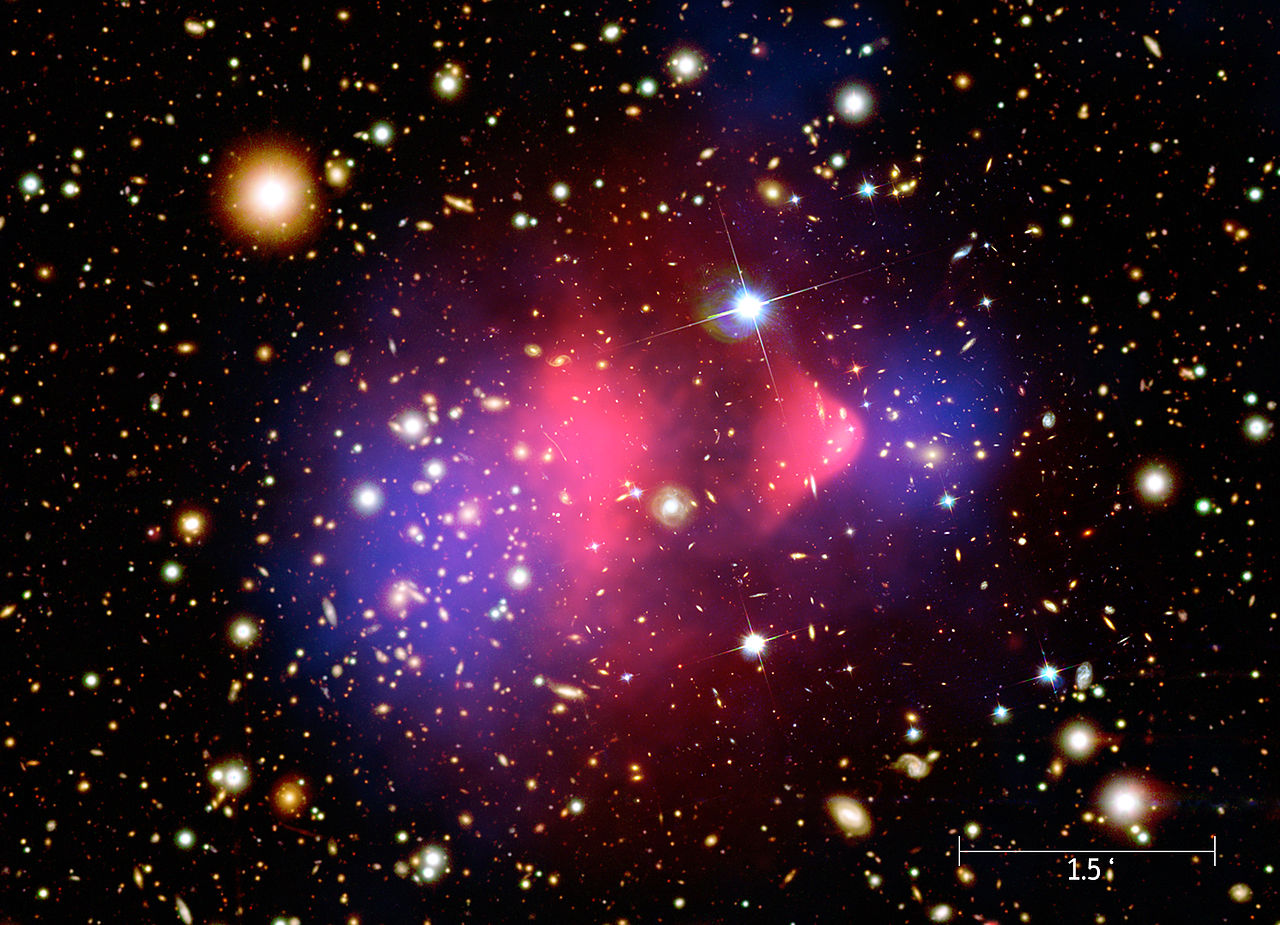
\includegraphics[width=0.6\textwidth]{plots/bulletcluster.jpg}
  \caption{Optical picture of the Bullet Cluster \cite{gravlens}. Two galaxy clusters collided, with the baryonic gas, here marked in red, being slowed down. The dark matter, here marked in blue, passed through and is visible through gravitational lensing.}
  \label{fig:gravlens}
\end{figure}

\noindent Measuring the rotation velocities of stars or gas as a function of their distance to the galaxy's core, also hints at a different type of matter. This is due to the fact, that visible matter itself would not be able to gravitationally bind objects of such high velocities at the observed distances to the galaxy. However adding an additional halo of (\textit{invisible}) matter could provide the necessary additional gravitational force.

As this new type of matter has only been observed indirectly through its effect on nearby structures, it cannot be emitting photons (hence the name \textit{dark} matter) or have a strong impact on cosmic rays. This leads to the assumption that only gravity and possibly the weak force may be couple to it. Other interactions\footnote{``Other interactions'' do not include the electromagnetic one, as this would lead to direct optical observation. However, possible interactions that have yet to be discovered are an option as well.} are also within the realms of possibility, but would also necessitate a coupling not stronger than the weak one. These requirements seem to fit the description of the neutrino, but as dark matter tends to cluster, its particles have to be massive and a lot slower.

One possible solution to the question what dark matter consists of are ``Weakly Interacting Massive Particles''. Often abbreviated as ``WIMPs''. The naming is self-explanatory. And while there are no candidates for this role in the Standard Model, supersymmetry does provide suitable particles. The most popular option amongst those, is the lightest supersymmetric particle or LSP, in case it is stable. As the mass hierarchy of supersymmetric particles can change depending on the parameters one chooses, there is not a set LSP. And while not all possible LSPs are considered WIMP candidates, some fit surprisingly well. Should supersymmetry be realized in nature and provide such an explanation for dark matter, it could solve one of the biggest mysteries in cosmology.



\subsubsection{The Hierarchy Problem}
\label{sec:hierprob}
Looking at the large differences in scales between the strength of the gravitational and the weak force (Tab.~\ref{tab:fundforces}), one inevitably expects to see new physics when approaching the point where gravity becomes non-negligible on a quantum level. Considering that the mass of the Higgs boson is of the order $\mathcal{O}(100\,\text{GeV})$ and couples to every massive particle, comparatively huge quantum corrections from heavy particles should contribute to its bare mass $\mu$ (Eq.~\ref{eq:higgslagrangian}). The Yukawa coupling to the Higgs field of an arbitrary fermion is given by

\begin{equation}
  \label{eq:yukawacoup}
  \mathcal{L}_{\text{Yukawa}} = - \lambda_f \bar{\psi} H \psi.
\end{equation}

\noindent Here, $\lambda_f$ denotes the coupling strength. The quantum loop correction of a fermion is depicted in figure~\ref{fig:higgsfloop}.

\begin{figure}[ht!]
  \centering
  \begin{subfigure}[b]{0.49\textwidth}
    \centering
    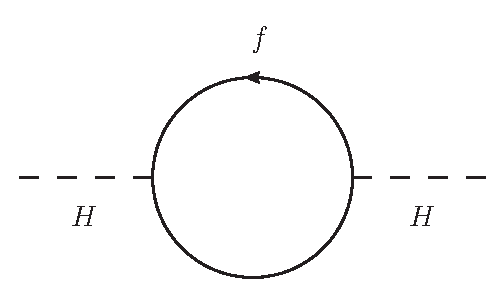
\includegraphics[width=0.6\textwidth]{plots/higgsfloop.pdf}
    \caption{}
    \label{fig:higgsfloop}
  \end{subfigure}
  \begin{subfigure}[b]{0.49\textwidth}
    \centering
    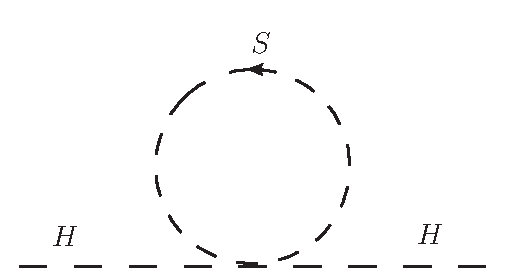
\includegraphics[width=0.6\textwidth]{plots/higgssloop.pdf}
    \caption{}
    \label{fig:higgssloop}
  \end{subfigure}
  \caption{Higgs boson with loop quantum corrections from a fermion \ref{fig:higgsfloop} and a scalar \ref{fig:higgssloop}}
\end{figure}

\noindent Calculating this Feynman diagram yields

\begin{equation}
  \label{eq:higgsfcorr}
  \Delta \mu = - \frac{|\lambda_f|^2}{8 \pi^2} \left[ \Lambda^2_{\text{UV}} + ... \right],
\end{equation}

\noindent where $\Lambda^2_{\text{UV}}$ is the ultraviolet momentum cut-off that is used to stop the loop integral from diverging. It can be interpreted as the scale at which one no longer expects the Standard Model to provide an accurate description of nature any more, meaning that new physics will enter the equation. Assuming this cut-off to be of a much larger scale, e.g. the Planck scale $M_{\text{P}} = 2.4 \cdot 10^{18}\,\text{GeV}$, this would result in corrections that go beyond 30 orders of magnitude when compared to the $\mathcal{O}(100\,\text{GeV})$ we expect for the Higgs' mass. The degree of precision necessary for this sort of parameter appears to be ``unnatural''.

However, in supersymmetry a scalar partner particle is introduced for every fermion, as well as a fermionic partner for every scalar particle. Assuming the couplings remain symmetrical $\lambda_S = |\lambda|^2$, both loop corrections (Fig. \ref{fig:higgsfloop} \& \ref{fig:higgssloop}) would cancel each other out, because fermions and bosons have opposite sign contributions.

\begin{equation}
  \label{eq:higgscancelcorr}
  \Delta \mu = \frac{1}{8 \pi^2} (\lambda_S - |\lambda_f|^2) \left[ \Lambda^2_{\text{UV}} + ... \right]
\end{equation}

\noindent This would provide a ``natural'' solution to the hierarchy problem and thus make supersymmetry all the more interesting.



\subsubsection{Gauge Coupling Unification}

Similarly to how the electromagnetic and weak force has been unified, the physics community has been looking to combine all four fundamental forces into one theory. As the individual forces show different behaviours at lower energy scales, they have to decouple at certain points. Since the coupling strength parameters $\alpha_i(Q),\ i = 1, 2, 3$ a function of the momentum transfer of the interaction, they intersect at certain energies. Figure \ref{fig:coupq} shows the evolution of $\alpha_i(Q)$ in both the Standard Model, as well as the minimal supersymmetric extension to it. 

\begin{figure}[ht!]
  \centering
  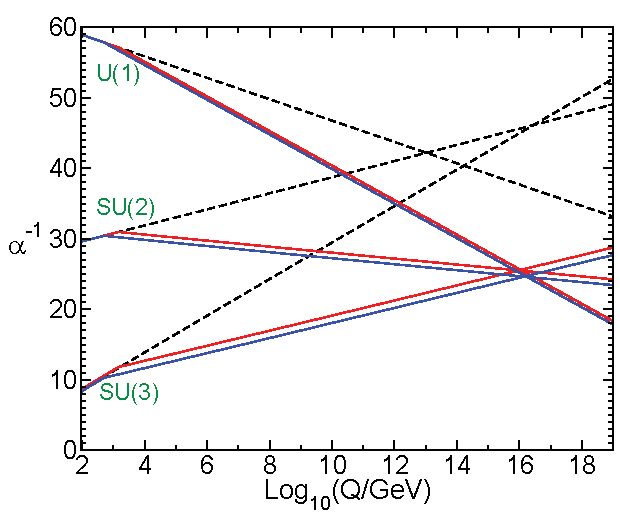
\includegraphics[width=0.6\textwidth]{plots/coupq.pdf}
  \caption{Exemplary evolutions of the inverse gauge couplings $\alpha^{-1}_i(Q)$ through renormalization group equations. The dashed lines show the Standard Model's prediction, while the coloured lines show the one of the Minimal Supersymmetric Standard Model.}
  \label{fig:coupq}
\end{figure}

As one can see, there is no possibility for unification of all three couplings within the Standard Model, while in the extension the points of intersection are in close proximity of each other. Taking the uncertainties of an extrapolation far beyond the reach of current experiments such as this into account, this could hint at an underlying ``grand unified theory'' (\textbf{GUT}). This GUT is, as the name suggests, the previously mentioned effort to unify all the fundamental forces and would be realized around an energy scale of roughly $\sim 10^{18}\,\text{GeV}$.



\subsection{The Minimal Supersymmetric Standard Model}

Symmetries play a huge role in physics. For example a translation in time results in the conservation of energy and a translation in space necessitates momentum to be conserved. In the case of supersymmetry, the quantum property of integer and half-integer spin is being considered as a symmetry. This means relating a fermion to a boson and vice versa. Mathematically speaking an operator that transforms a fermionic state into a bosonic one and back, has to be introduced.

\begin{equation}
  \label{eq:fermiboso}
  Q \Ket{Fermion} = \Ket{Boson}; \quad Q \Ket{Boson} = \Ket{Fermion}
\end{equation}

The new states, which relate to a Standard Model particle each, are called superpartners. As a naming scheme for the partner-particles, the following rules apply. Adding \textit{s-} as a prefix to a fermionic particle's name, yields the title for the scalar superpartner. Using the electron as an example, one gets the selectron. Likewise for scalar particles and their superpartners, the name has to be extended by the suffix \textit{-ino}. The Higgs boson's counterpart would be the Higgsino.

The ``MSSM'', short for ``Minimal Supersymmetric Standard Model'', is the most commonly used and widely studied implementation of supersymmetry. The ``minimal'' expresses itself in the amount of superpartners added to the Lagrangian, which has been kept to the necessary minimum. Usually this means one superpartner for every left-handed and another one for every right-handed particle, which are then sorted into supermultiplets. The Standard Model's Higgs boson is insufficient for the MSSM, as adding just its superpartner would lead to an anomaly in the electroweak gauge symmetry. Thus the number of Higgs eigenstates, as well their supersymmetric counterparts, are extended to four. The supermultiplets of the MSSM are shown in table~\ref{tab:mssmmult}.

\begin{table}[ht!]
  \centering
  \begin{tabular}{| l | c | c | c |}
    \hline
    \multicolumn{2}{ |c| }{ Names }                     & Spin 0        & Spin 1/2 \\ \hline \hline
    \multirow{3}{2.5cm}{(s)quarks $\times 3$~families}  & $Q$           & $\left(\tilde{u}_L \ \tilde{d}_L \right)$     & $\left(u_L \ d_L \right)$ \\
                                                        & $\bar{U}$     & $\tilde{u}_R$                                 & $u_L$ \\
                                                        & $\bar{D}$     & $\tilde{d}_R$                                 & $d_R$ \\ \hline
    \multirow{2}{2.5cm}{(s)leptons $\times 3$~families} & $L$           & $\left(\tilde{\nu}_e \ \tilde{e}_L \right)$   & $\left(\nu_e \ e_L \right)$ \\
                                                        & $\bar{E}$     & $\tilde{e}_R$                                 & $e_R$ \\ \hline
    \multirow{2}{*}{Higgs (-inos)}                      & $H_u$         & $\left(H^+_u \ H^0_u \right)$                  & $\left(\tilde{H}^+_u \ \tilde{H}^0_u \right)$ \\
                                                        & $H_d$         & $\left(H^0_d \ H^-_d \right)$                  & $\left(\tilde{H}^0_d \ \tilde{H}^-_d \right)$ \\ \hline \hline
    \multicolumn{2}{ |l| }{}                            & Spin 1/2      & Spin 1 \\ \hline
    \multicolumn{2}{ |l| }{gluino, gluon}               & $\tilde{g}$   & $g$ \\
    \multicolumn{2}{ |l| }{W (-ino)}                    & $\tilde{W}^{\pm}, W^0$   & $W^{\pm}, W^0$ \\
    \multicolumn{2}{ |l| }{B (-ino)}                    & $\tilde{B}^0$ & $B^0$ \\ \hline
  \end{tabular}
  \caption{Supermultiplets of the Minimal Supersymmetric Standard Model. Left-handed particles are sorted into doublets and right-handed ones into singlets.}
  \label{tab:mssmmult}
\end{table}

Similarly to how the gauge eigenstates $W^i_\mu$ and $B^0_\mu$ mix to their respective mass eigenstates, the mass eigenstates for the MSSM particles also don't always coincide with a single gauge eigenstate. For the first two families of both the sleptons and squarks the mixing is assumed to be negligible. The charged components of the third family however, do have different mass and gauge eigenstates:

\begin{align}
  \label{eq:3fammix}
  \tilde{t}_L \tilde{t}_R & \xrightarrow{\text{\tiny{Mixing}}} \tilde{t}_1 \tilde{t}_2 \\
  \tilde{b}_L \tilde{b}_R & \xrightarrow{\text{\tiny{Mixing}}} \tilde{b}_1 \tilde{b}_2 \\
  \tilde{\tau}_L \tilde{\tau}_R & \xrightarrow{\text{\tiny{Mixing}}} \tilde{\tau}_1 \tilde{\tau}_2
\end{align}

\noindent While in this case the amount of particles remains identical, the electroweak and Higgs gauge bosinos' mass eigenstates can only be sorted by their mass hierarchy and charge:

\begin{align}
  \label{eq:ewhsusymix}
  \tilde{B}^0 \tilde{W}^0 \tilde{H}^0_u \tilde{H}^0_d & \xrightarrow{\text{\tiny{Mixing}}} \tilde{\chi}^0_i \quad \text{with} \quad i = 1,2,3,4 \\
  \tilde{W}^\pm \tilde{H}^+_u \tilde{H}^-_d & \xrightarrow{\text{\tiny{Mixing}}} \tilde{\chi}^\pm_i \quad \text{with} \quad i = 1,2
\end{align}

\noindent As the MSSM also requires new ``Standard Model'' Higgs bosons, these also mix:

\begin{equation}
  \label{eq:hmix}
  H^0_u H^0_d H^+_u H^-_d \xrightarrow{\text{\tiny{Mixing}}} h^0 H^0 A^0 H^\pm
\end{equation}

\noindent The $h^0$ resembles the Standard Model's Higgs closely and therefore the potential Higgs discovery from section~\ref{sec:higgs} does not stand in direct conflict with the MSSM. Gluons and gluinos do not mix.

With the given particle content, the final step of the implementation is modifying the Lagrangian. Integration of the supersymmetric extension into it, requires the superpotential with the respective superfields from table~\ref{tab:mssmmult} to be added.

\begin{equation}
  \label{eq:mssmsuperpot}
  W_{\text{MSSM}} = \bar{U} \mathbf{y_u} Q H_u - \bar{D} \mathbf{y_d} Q H_d - \bar{E} \mathbf{y_e} L H_d + \mu H_u H_d
\end{equation}

\noindent The $\mathbf{y_i}$ with $i = u,d,e$ are the Yukawa coupling parameters. They are $3 \times 3$ matrices in flavour space and determine the mass spectrum. The $\mu$-term is the supersymmetric version of the $\mu$-term in the Higgs mechanism's superpotential (Eq.~\ref{eq:higgslagrangian}).

\subsection{Soft SUSY Breaking}

With the current assumption that supersymmetry is an exact symmetry, in particular sparticle masses being identical to their Standard Model counterpart, the lack of discoveries of at least the low mass components (e.g. the selectron) necessitates a spontaneously broken symmetry. This means that the supersymmetric partner particles are expected to have masses which are outside the reach of current experiments. One also has to keep in mind, that the ``naturalness'' of the solution to the hierarchy problem (Sec.~\ref{sec:hierprob}) depends on the coupling strengths being equal. To allow the symmetry to be broken while keeping the cancellation of the loop contributions to the Higgs mass, requires the symmetry breaking to be \textit{soft}. This means that the Lagrangian can be written like

\begin{equation}
  \label{eq:softlagr}
  \mathcal{L} = \mathcal{L}_{\text{SUSY}} + \mathcal{L}_{\text{soft}},
\end{equation}

\noindent to split the gauge and Yukawa couplings (SUSY) from the mass terms (soft).


To achieve this distinct shape of the Lagrangian, a new interaction is necessary for which various models have been suggested. \textit{Gravity mediated supersymmetry breaking}, also known as \textit{Planck-scale supersymmetry breaking}, is the most popular one. The general idea is that, through the new physics that enter once gravity becomes relevant on a quantum scale, new gauge bosons mediate the masses of the supersymmetric particles. By requiring supersymmetry to be a local gauge symmetry, similarly to how the electroweak and strong force are implemented, one receives both a graviton (Spin 2) and a gravitino (Spin 3/2). It also yields an additional term for the goldstino, which is absorbed by the gravitino. The latter acquires mass due to the absorption. This theory is called supergravity.

\subsubsection{Constrained Minimal Supersymmetric Standard Model}

The most simple version of supergravity with the least amount of additional particles is called \textit{minimal supergravity} (\textbf{mSUGRA}) or \textit{constrained Minimal Supersymmetric Standard Model} (\textbf{cMSSM}). One of the reasons why this particular realization is popular, is the massive reduction of free parameters it achieves. While there are 105 of them in the MSSM, the scale dependency of the sparticle masses allows for a unification of multiple parameters at the grand unified theory (\textbf{GUT}) scale. Figure~\ref{fig:msugrarge} displays how the individual scalar and fermionic masses converge at the respective points of intersection.

\begin{figure}[ht!]
  \centering
  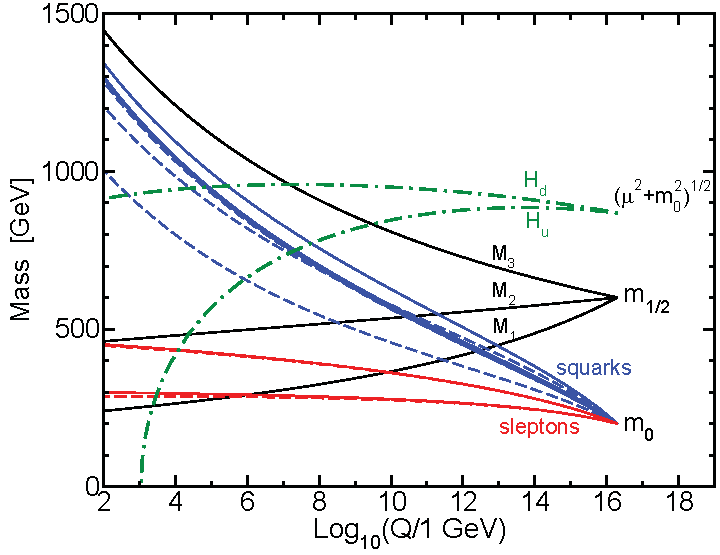
\includegraphics[width=0.7\textwidth]{plots/msugrarge.pdf}
  \caption{Unification of sparticle masses at the GUT scale in the cMSSM, thus allowing for a significantly smaller amount of free parameters.}
  \label{fig:msugrarge}
\end{figure}

\noindent Through the renormalization group equations, it is possible to extrapolate from these points. The remaining 5 parameters are:

\begin{itemize}
\item $m_0$ - Universal mass of scalar sparticles at the GUT scale
\item $m_{1/2}$ - Universal mass of fermionic sparticles at the GUT scale
\item $A_0$ - Trilinear Higgs coupling strength at the GUT scale
\item $\tan{\beta}$ - Tangents of the ratio of the vacuum expectation values of $H^0_u$ \& $H^0_d$
\item $\text{sgn}\,\mu$ - The sign of the bilinear Higgsino mixing parameter
\end{itemize}

\subsection{R-Parity}

When adding the most general version superpotential for the MSSM to the Lagrangian, the theory appears to be consistent at first. However, certain phenomenological discrepancies would be left unaddressed. There are lepton number violating (\textbf{LNV}), as well as baryon number violating (\textbf{BNV}) terms:


\begin{align}
  \label{eq:lnvlagr}
  W_{\text{LNV}} &= \frac{1}{2} \lambda_{ijk} L_i L_j \bar{E}_k + \lambda^\prime_{ijk} L_i Q_j \bar{D}_k + \kappa^{i} L_i H_u \\
  \label{eq:bnvlagr}
  W_{\text{BNV}} &= \frac{1}{2} \lambda^{\prime\prime}_{ijk} \bar{U}_i \bar{D}_j \bar{D}_k
\end{align}


\noindent Here $\lambda$, $\lambda^\prime$, $\lambda^{\prime\prime}$ and $\kappa$ denote the coupling strengths of the the respective interactions between the superfields (see tab.~\ref{tab:mssmmult}). The indices $i$, $j$, and $k$ represent family numbers. These terms would for example lead to rapid proton decay. The latter has an experimental limit at $90\pct$ confidence level of $6.6 \cdot 10^{33}$ years, given by the Super-Kamiokande experiment in Japan~\cite{protondecay}.

To prevent this inconsistency, both types of terms could be suppressed by simply assuming the coupling parameters to be equal to zero. However in the MSSM, instead of simply forcing the theory to adhere to the observation through demanding certain parameters to be set, a new symmetry is introduced. The so called ``$R$-parity'' $P_R$ is a discreet $Z_2$ symmetry and assigns a quantum number to every particle, which can be calculated as by:

\begin{equation}
  \label{eq:rparity}
  P_R = (-1)^{3 (B-L) + 2 S}
\end{equation}

\noindent One can easily confirm that every particle has an even $R$-parity ($P_R = +1$), while the supersymmetric counterparts have an odd $R$-parity ($P_R = -1$). Assuming $R$-parity is conserved, supersymmetric particles can only be produced in even numbers (usually pairs). This is due to it being a multiplicative quantum number, which calculates as follows for a vertex. With two particles entering one gets $P_R = (+1) \cdot (+1) = +1$. If they annihilate and produce two sparticles the calculation yields $P_R = (-1) \cdot (-1) = +1$. Obviously under $R$-parity conservation, this could not have produced one sparticle alongside one particle. This also forbids both the lepton and baryon number violating processes (Eq.~\ref{eq:lnvlagr}~\&~\ref{eq:bnvlagr}) and has another major phenomenological consequence. The lightest supersymmetric particle (\textbf{LSP}) has to be stable, as any further decay would require an additional, even lighter supersymmetric particle. Should this LSP be neutral, it would only interact very weakly with baryonic matter. Under these circumstances, supersymmetry could provide a suitable candidate for a WIMP (compare to section~\ref{sec:dm}).



\subsubsection{The Violation of R-Parity}
\label{sec:rparityvio}

While most supersymmetric models do make use of $R$-parity, there is no intrinsic motivation for choosing this symmetry over others who can provide the same phenomenology. It can be shown that there are other, gauge anomaly free $Z_N$ symmetries that can prevent the proton from decaying~\cite{b3p6}. In this analysis baryon-triality $B_3$ is assumed. The discreet symmetry for this scenario is given by~\cite{b3def}

\begin{equation}
  \label{eq:b3symmetry}
  \psi_j \rightarrow e^{\alpha_j 2\pi i/3} \psi_j.
\end{equation}

\noindent The values of $\alpha_j$ for the respective superfields are given in table~\ref{tab:alphaj} below.

\begin{table}[htb]
  \centering
  \begin{tabular}{|c|c|c|c|c|c|c|c|}
    \hline
    & $Q_i$ & $\bar{U}_i$ & $\bar{D}_i$ & $L_i$ & $\bar{E}_i$ & $H_d$ & $H_u$ \\ \hline
    $\alpha_j$ & 0 & 2 & 1 & 2 & 2 & 2 & 1 \\ \hline
  \end{tabular}
  \caption{Values of $\alpha_j$ for the respective superfields in the baryon-triality model.}
  \label{tab:alphaj}
\end{table}

Baryon-triality allows for the lepton number violating terms (Eq.~\ref{eq:lnvlagr}), but forbids baryon number violating ones (Eq.~\ref{eq:bnvlagr}). As a result the proton remains stable, while the LSP is able to decay. Due to the instability of the LSP in RPV supersymmetry, the idea of an LSP being a WIMP candidate has to be abandoned. However, resonant production of sleptons is possible, which can lead to very distinct decay chains (without ``invisible'' particles). This analysis will make use of that.


\subsection{Analysis Model}
\label{sec:anamodel}

As this analysis is focussing on searching for resonant production of sleptons, R-parity has to be violated (cf. sec.~\ref{sec:rparityvio}). To determine the viaable couplings through which sleptons (Eq.~\ref{eq:lnvlagr}) can be produced, one has to keep the initial state in mind. For proton-proton collisions this strongly favours the LQD term with $\lambda^\prime_{ijk}$, as it is able to convert two quarks directly into a slepton. With the valence quarks of a proton being of the first generation, their contribution to the coupling will be dominant. While this sets $j = k = 1$, the remaining index determines the generation of the sleptons. Since neutrinoless double beta decay puts strict bounds on the coupling for the first generation $\lambda^\prime_{111}$~\cite{rpvimpl}, searching for the second generation is the more attractive option. Assuming single coupling dominance~\cite{rpvimpl} for $\lambda^\prime_{211}$, contributions from other couplings can be neglected.

\subsubsection{Current Limits}

While $R$-parity conserving scenarios are more popular and therefore more thoroughly investigated, there has also been searches for the particular model this analysis concerns itself with. As none of these searches have had any discoveries, their main results are limits on the value of $\lambda^\prime_{211}$.

\begin{figure}[ht!]
  \centering
  \begin{subfigure}[b]{0.495\textwidth}
    \centering
    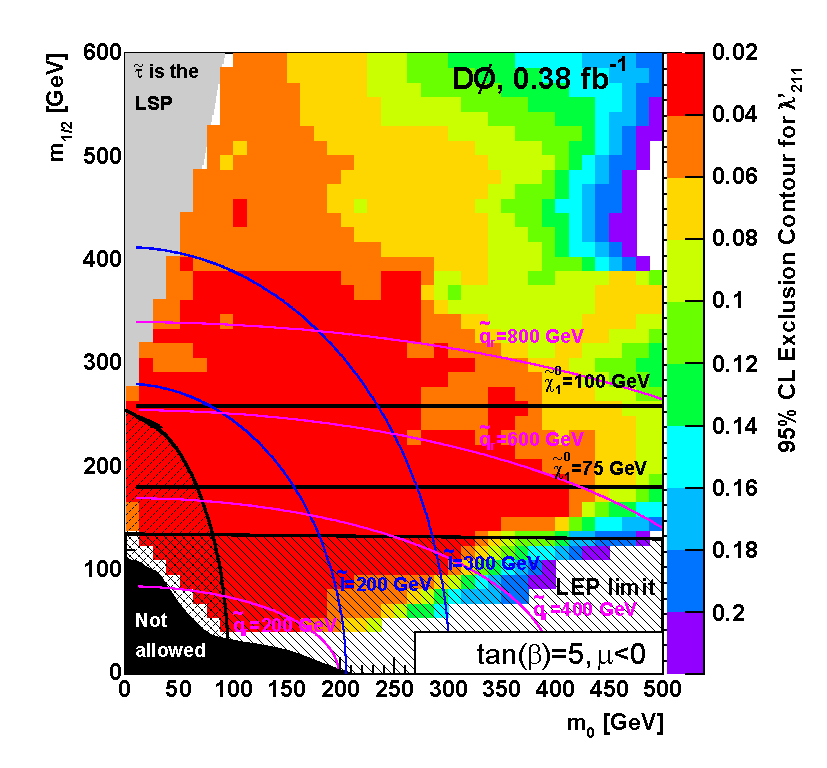
\includegraphics[width=\textwidth]{plots/auterrpv.pdf}
    \caption{\label{fig:auterrpv}}
  \end{subfigure}
  \begin{subfigure}[b]{0.495\textwidth}
    \centering
    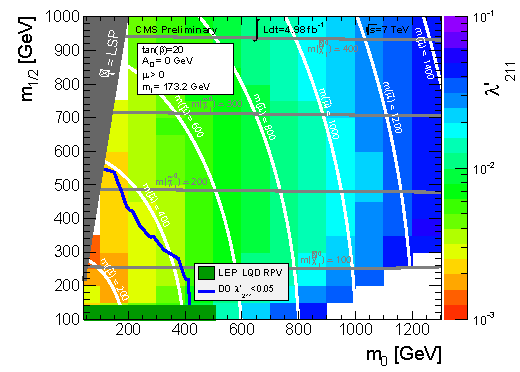
\includegraphics[width=\textwidth]{plots/endresrpv.pdf}
    \caption{\label{fig:endresrpv}}
  \end{subfigure}
  \caption{$95\,\%$ C.L. exclusion limits for resonant slepton production through the $\lambda^{\prime}_{211}$ coupling. They have been calculated using the data measured at the D0 experiment (\ref{fig:auterrpv}) at the Tevatron~\cite{auter} and the measurements of CMS experiment at the LHC during 2011, which was operating at a center-of-mass energy of $\sqrt{s} = 7\,\text{TeV}$~\cite{endres}.}
\end{figure}

Figure~\ref{fig:auterrpv} shows the results from the D0 experiment at the Tevatron~\cite{auter,d0rpv}, which were the most stringent limits from a collider experiment prior to the LHC. Shown are the $95\pct$ confidence level exclusion limits that this direct search yielded.

Due to the technically more advanced combination of the LHC and CMS experiment, the results could be expanded upon. Figure~\ref{fig:endresrpv} shows the extended, more strict limits, which were obtained using the data recorded during 2011~\cite{endres}. These exclusion ranges are the basis for this analysis.


%%% Local Variables: 
%%% mode: latex
%%% TeX-master: "document"
%%% End: 
